As described in \ref{Sec:Theory_X-ray_diffraction}, constructive interference of incoming and scattered X-rays may give insight in the symmetry of exposed crystal structures.
This can be utilized for thin film investigation and is called \gls{XRD}.
The \gls{XRD} device used for this work, namely an \textit{X'Pert Pro} (\textit{Malvern Panalytical Ltd.}), as well as the applied scanning techniques will be presented in the following.

A sample with surface normal parallel to the $z$-axis of the laboratory system is exposed with X-rays at an angle $\omega$ between sample surface and incident radiation.
The diffracted radiation is measured at an angle $\alpha_\mathrm{out}$ between sample surface and detector.
$2\theta$ is used to describe the angle between outgoing beam and the extension of the incoming beam, which both span the scattering plane.
It follows that $2\theta=\omega+\alpha_\mathrm{out}$.
Note that $\theta$ in Equ.~(\ref{Equ:Theory_BraggCondition}) is the same angle as half of $2\theta$.
The scattering plane is depicted in Fig.~\ref{Fig:Methods_XRD_geometry}a.
The sample can be rotated by $\phi$ (\enquote{azimuth}) and $\psi$ around an axis parallel to the surface normal and parallel to the intersection of sample surface and scattering plane, respectively.

% ---
\subsection{2\texttheta-\textomega-scans}
    \label{Sec:Methods_2ThetaOmega}
% ---
\begin{figure}
    \centering
    \begin{tabular}{ll}
        \textbf{(a)}&\textbf{(b)}\\
        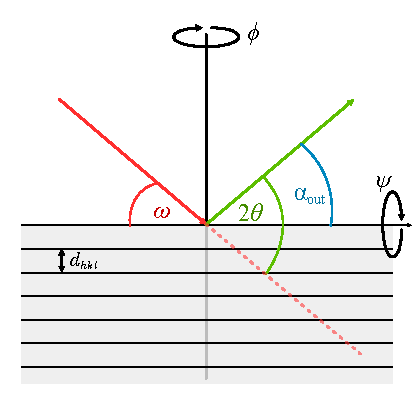
\includegraphics{theta-omega-noTilt.pdf}
        &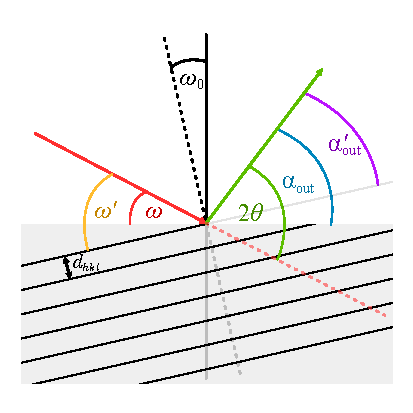
\includegraphics{theta-omega-Tilt.pdf}
    \end{tabular}
    \caption{\textbf{(a)} Geometry for a 2\texttheta-\textomega-scan without offset. \textbf{(b)} Scattering geometry containing an offset $\omega_0$. Angle of incidence and angle of diffraction decrease and increase, respectively. Note that $2\theta$ is not affected by this offset.}
    \label{Fig:Methods_XRD_geometry}
\end{figure}
When probing for lattice plane distances using the \gls{bc} in its simplest form, it is assumed that the scattering planes are parallel to the sample surface (cf. Fig.~\ref{Fig:Methods_XRD_geometry}a).
It is necessary that $\omega=\alpha_\mathrm{out}$ which implies $2\theta=2\omega$.
So the angle of incidence $\omega$ is coupled to $2\theta$ which represents the distance between lattice planes (cf. Equ.~(\ref{Equ:Theory_BraggCondition})).
Measuring the diffracted X-ray intensity while varying $2\theta$ and maintaining the condition $2\theta=2\omega$, is called a 2\texttheta-\textomega-scan.
This results in a so-called 2\texttheta-\textomega\ diffraction pattern, where peaks correspond to constructive interference and thus to certain lattice plane distances.

When analyzing 2\texttheta-\textomega\ diffraction patterns, one usually compares to predicted peak positions of the expected phase of the compound which is investigated.
This reference diffraction pattern stems from powder samples of the respective compound, containing all crystal orientations during one 2\texttheta-\textomega-scan.
When a peak is identified, a possible peak shift is determined and the shape of the peak is investigated.
Peak shifts may be due to residual stress, substrate induced strain or compositional gradients in the thin film 
    \cite{harrington2021}.
A minimum amount of peak broadening is always present due to convergence of the incident beam as well as convolution of K\textalpha\textsubscript{1}- and K\textalpha\textsubscript{2}-radiation (cf.~\ref{Sec:Theory_XRays}), which is called instrumental broadening
    \cite{harrington2021}.
The \gls{FWHM} of the highly crystalline substrate peaks may give a reference for broadening of peaks in 2\texttheta-\textomega\ diffraction data.  

This method can be extended to measure lattice planes which are not parallel to the sample surface but tilted by $\omega_0$.
This is done by rotating the reference frame of the sample in such a way that the \gls{bc} is fulfilled again.
Note that $2\theta$ does not change upon rotation, as can be seen in Fig.~\ref{Fig:Methods_XRD_geometry}b.
When probing for plane distances of the rotated lattice, one finds for the coupling between $2\theta$ and $\omega$:
\begin{align*}
    \omega'&=\alpha_\mathrm{out}'\\
    \omega+\omega_0&=\alpha_\mathrm{out}-\omega_0\\
    \omega+\omega_0&=(2\theta-\omega)-\omega_0\\
    \Rightarrow 2\theta&=2(\omega+\omega_0)=2\omega'\,.
\end{align*}
This coupling is equivalent to a 2\texttheta-\textomega-scan but with an offset $\omega_0$ applied to the angle of incidence.
There are several use cases for applying an offset $\omega_0$:
\begin{enumerate}[label=(\roman*)]
    \item It is assumed that $\omega$ denotes the angle between incident X-ray beam and the sample surface.
    But a perfect alignment between sample and sample holder is not always possible.
    So to correct this tilt between expected sample position and it's real inclination, the offset $\omega_0$ can be set to really probe for lattice planes parallel to the sample surface.
    This is done before measuring a 2\texttheta-\textomega-scan to achieve preciser results.
    \item When probing for lattice planes which are not parallel to the sample surface (\enquote{asymmetric reflections}), one can apply the expected inclination angle as an offset $\omega_0$.
    This is the case in Fig.~\ref{Fig:Methods_XRD_geometry}b.
    \item When $2\theta$ is fixed, but $\omega_0$ is varied, a so-called \textomega-scan is performed, which enables quantification of mosaicity (cf.~\ref{Sec:Methods_omegaScan}).
\end{enumerate}

% ---
\subsection{\textomega-scans}
    \label{Sec:Methods_omegaScan}
% ---
Thin films may exhibit a distribution of lattice plane inclination, called mosaicity.
This results in an observation of diffraction peaks for several offsets $\omega_0$.
The mosaicity can thus be quantified by fixing $2\theta$, representing a certain lattice plane distance, and then vary $\omega_0$ and measure the X-ray intensity.
This is called an \textomega-scan, and the \gls{FWHM} of the observed diffraction pattern (also called \enquote{Rocking curve}) is a measure for the mosaicity
    \cite{harrington2021}.
\textomega-scans are particularly useful when comparing a set of thin films of varying deposition parameters to optimise growth conditions.
In particular, recording Rocking curves of symmetric and asymmetric lattice planes allows the calculation of dislocation densities in the thin film
    \cite{srikant1997}.
% ---
\subsection{\textphi-scans}
    \label{Sec:Methods_phiScan}
% ---
A 2\texttheta-\textomega-scan is not capable of resolving in-plane rotations of crystal domains, because the distance of lattice planes parallel to the surface are not affected.
Those rotational domains can be detected by probing for lattice planes which are inclined with respect to the surface, i.e.\ by fixing $2\theta$ to the expected lattice plane distance and $\omega_0$ to the inclination angle (cf. Fig.~\ref{Fig:Methods_XRD_geometry}b).
Depending on the symmetry of the inspected material, constructive interference should only appear for distinct values of $\phi$.
So by rotating the sample by \qty{360}{\degree} and simultaneously recording the X-ray intensity, a so-called \textphi-scan (also called \enquote{Azimuth-scan}) can yield information about the existence of rotational domains.
If the number of observed peaks in the \textphi-scan diffraction pattern exceeds the theoretically expected number for a single crystal, rotational domains are present
    \cite{harrington2021}.
Furthermore, comparing the \textphi-scan diffraction data of thin film and substrate reveals whether the film has grown with an in-plane rotation with respect to the substrate.
Finally, if the thin film grows in a tilted manner on the substrate, a \textphi-scan prior to an \textomega-scan can ensure the correct positioning bevor alignment.
Then, the \gls{bc} is fulfilled for performing a 2\texttheta-\textomega-scan.

% ---
\subsection{Reciprocal Space Maps}
    \label{Sec:Methods_RSM}
% ---
Because the \gls{bc} is equal to the description of diffraction with $\mathbf{k}'-\mathbf{k}$ and reciprocal space vectors $\mathbf{K}_{hkl}$ (cf.~\ref{Sec:Theory_X-ray_diffraction}), both can be used depending on context.
Henceforth, $\mathbf{k}'-\mathbf{k}$ will be denoted by the \enquote{scattering vector} $\mathbf{q}$.
Note that $\mathbf{k}$ and $\mathbf{k}'$ are parallel to incoming and outcoming beam, respectively.
From the definition of angles, it follows that
\begin{align}
    \mathbf{q}
    =\begin{pmatrix}
        q_\parallel\\
        q_\perp
    \end{pmatrix}
    &=\mathbf{k}'-\mathbf{k}\\
    &=\frac{1}{\lambda}
    \begin{pmatrix}
        \cos\alpha_\mathrm{out}\\
        \sin\alpha_\mathrm{out}
    \end{pmatrix}
    -\frac{1}{\lambda}
    \begin{pmatrix}
        \cos\omega\\
        -\sin\omega
    \end{pmatrix}\\
    &=\frac{1}{\lambda}
    \begin{pmatrix}
        \cos(2\theta-\omega)-\cos(\omega)\\
        \sin(2\theta-\omega)+\sin(\omega)
    \end{pmatrix}\,.
    \label{Equ:Methods_qDef}
\end{align}
From Equ.~(\ref{Equ:Methods_qDef}), two properties follow for the scattering vector:
\begin{align}
    -q_\parallel/q_\perp&=-\tan\left(\omega-\frac{2\theta}{2}\right)=\tan\omega_0
        \label{Equ:Methods_qDir}\,,\\
    \left|\mathbf{q}\right|&=\sqrt{q_\parallel^2+q_\perp^2}=\frac{1}{\lambda}2\sin\theta\overset{\mathrm{Bragg}}{=}\frac{1}{d_{hkl}}\,,
    \label{Equ:Methods_qAbs}
\end{align}
where the last equality of Equ.~(\ref{Equ:Methods_qAbs}) holds, if $\mathbf{q}$ is a reciprocal lattice vector $\mathbf{K}_{hkl}$.
The scattering vector, together with the corresponding \gls{XRD} geometry is depicted in Fig.~\ref{Fig:Methods_qDef}a.
\begin{figure}
    \centering
    \begin{tabular}{ll}
        \textbf{(a)}&\textbf{(b)}\\
        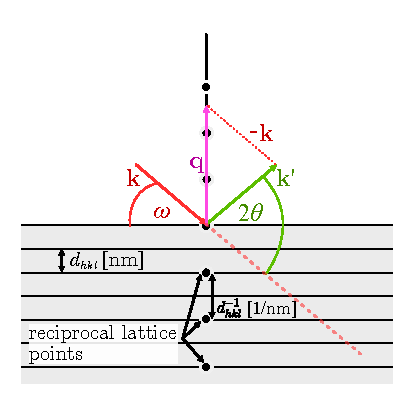
\includegraphics{reciprocalDef.pdf}
        &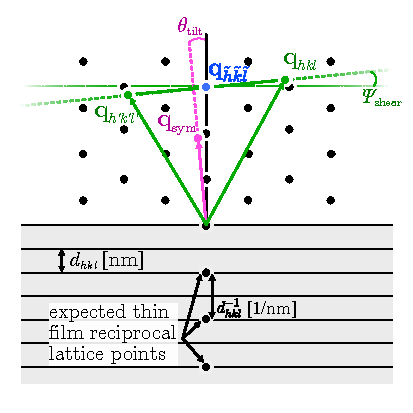
\includegraphics{correctReciprocal.pdf}
    \end{tabular}
    \caption{\textbf{(a)} Construction of the scattering vector (magenta) from incoming (red) and outgoing (green) beam, according to Equ.~(\ref{Equ:Methods_qDef}).
    The reciprocal lattice points are visualized together with the lattice planes.
    It has to be noted that the distances between lattice planes and between reciprocal lattice points have different dimensions.
    \textbf{(b)}}
    \label{Fig:Methods_qDef}
\end{figure} 
Because $2\theta$ and $\omega$ can simultaneously be represented by $\mathbf{q}$, it is possible to measure intensities for several $\mathbf{q}$, such that a part of the reciprocal space $Q\ni\mathbf{q}$ is mapped.
Consequently, this is called a \gls{RSM}.
According to Equ.~(\ref{Equ:Theory_ConstructiveInterference}), a peak in 2D reciprocal space $Q$ should be observed if $\mathbf{q}$ is a reciprocal space vector.
In this case, $\mathbf{q}=\mathbf{K}_{hkl}$ is called a \enquote{reflection}.
With Equ.~(\ref{Equ:Methods_qDir}) one can determine $\omega_0$ -- the direction of the corresponding lattice planes\footnote{
    Note that the \enquote{$-$} in $-q_\parallel/q_\perp$ is necessary, such that this fraction is the tangens the angle between $\mathbf{q}$ and surface normal with correct sense of rotation. 
}, and with Equ.~(\ref{Equ:Methods_qAbs}) the lattice plane distance $d_{hkl}$ can be calculated.

A 2\texttheta-\textomega-scan corresponds to a set of $\mathbf{q}$ with fixed direction in reciprocal space, but varying length.
For scanning symmetric reflections, $\mathbf{q}$ is parallel to the surface normal (as in Fig.~\ref{Fig:Methods_qDef}a).
On the other hand, an \textomega-scan corresponds to a set $\mathbf{q}$ with fixed length but varying direction.
The mosaicity can therefore approximately quantified by the broadening of a reflection perpendicular to the direction of $\mathbf{K}_{hkl}$.
Because anisotropic strain has an effect on direction and length of inclined lattice planes, asymmetric reflections, i.e.\ $\omega_0\neq0$, can be deconvoluted into an in-plane and out-of-plane component.
By this means, \glspl{RSM} enable the calculation of lattice constants.
To precisely calculate the latter, several corrections are applied to the recorded \glspl{RSM}, as proposed in \textcite{kneiss2021}:
\begin{enumerate}
    \item High-quality sapphire substrates are used for deposition of thin films.
    It can be assumed that they have the expected crystal structure of bulk \textalpha-\ce{Al2O3} (cf. Tab.~\ref{Tab:sesquiLatticeConstants}).
    So any deviation of the observed reflection $\mathbf{q}_{hkl}^\mathrm{\ce{Al2O3},obs}$ from the expected peak position $\mathbf{q}_{hkl}^\mathrm{\ce{Al2O3},lit}$ is corrected by a rotation $\mathbf{R}$ and scaling $\rho$ of reciprocal space $Q$:
    \begin{equation}
        \mathbf{q}^\mathrm{cor}=\rho\mathbf{R}\cdot\mathbf{q}^\mathrm{obs}\quad,\quad\mathbf{q}^\mathrm{obs}\in Q\,,
    \end{equation}
    with
    \begin{align}
        \label{Equ:Methods_rotation}
        \mathbf{R}&=\begin{pmatrix}
            \cos\gamma&-\sin\gamma\,,\\
            \sin\gamma&\cos\gamma
        \end{pmatrix}\quad,\quad
        \gamma=\arccos\left(
            \frac
                {\mathbf{q}_{hkl}^\mathrm{\ce{Al2O3},lit}
                    \cdot\mathbf{q}_{hkl}^\mathrm{\ce{Al2O3},obs}}
                {\left|\mathbf{q}_{hkl}^\mathrm{\ce{Al2O3},lit}\right|
                    \cdot\left|\mathbf{q}_{hkl}^\mathrm{\ce{Al2O3},obs}\right|}
            \right)\\
        \rho&=\frac{\left|\mathbf{q}_{hkl}^\mathrm{\ce{Al2O3},lit}\right|}{\left|\mathbf{q}_{hkl}^\mathrm{\ce{Al2O3},obs}\right|}\,.
    \end{align}

    \item If the thin film grows tilted (e.g.\ due to slip systems, cf.~\ref{Sec:Theory_Relaxed}), a symmetric reflection -- having scattering vector parallel to the surface normal in theory -- will exhibit an in-plane component $q_{\parallel,hkl}^\mathrm{film}\neq0$.
    The tilt angle can be calculated by Equ.~(\ref{Equ:Methods_qDir}): 
    \begin{equation}
        \theta_\mathrm{tilt}=\arctan\left(-\frac{q_{\parallel,hkl}^\mathrm{film}}{q_{\perp,hkl}^\mathrm{film}}\right)\,.
    \end{equation}
    To determine the lattice constants from asymmetric peaks, the reciprocal space is again rotated as in Equ.~(\ref{Equ:Methods_rotation}) but with rotation angle $-\theta_\mathrm{tilt}$.
    This scenario is depicted in Fig.~\ref{Fig:Methods_qDef}b, where the magenta colored reflection deviates from the expected symmetric position.

    \item If the thin film is sheared, a symmetric reflection $\mathbf{q}_{\tilde{h}\tilde{k}\tilde{l}}^\mathrm{film}$ will be unaffected.
    On the contrary, an asymmetric reflection with both in- and out-of-plane component is affected.
    To get reliable results for the lattice constants, this shear angle $\Psi_\mathrm{shear}$ has also to be corrected, and can be calculated from two inclined lattice planes ($hkl$) and ($h'k'l'$), i.e.\ scattering vectors with non-zero in-plane component.
    Those vectors must have symmetry of a mirror plane perpendicular to the scattering plane\footnote{
        This can be achieved by probing for a plane ($hkl$) and then rotate the sample around $\phi$ by \qty{180}{\degree}.
    }.
    The geometry is depicted in Fig.~\ref{Fig:Methods_qDef}b, with the blue and green reflections representing the symmetric and asymmetric reflections, respectively.
    The shear angle can be calculated with
    \begin{equation}
        \Psi_\mathrm{shear}=\arctan\left(\frac{
            q_{\perp,hkl}^\mathrm{film}
            -q_{\perp,h'k'l'}^\mathrm{film}
        }{
            q_{\parallel,hkl}^\mathrm{film}
            -q_{\parallel,h'k'l'}^\mathrm{film}
        }\right)\,.
    \end{equation}
    To correct the shear, a rotation around the corresponding symmetric reciprocal lattice point $\mathbf{q}_{\tilde{h}\tilde{k}\tilde{l}}^\mathrm{film}$ with the same expected out-of-plane component must be applied.
\end{enumerate}

\subsection{Technical Aspects}
The radiation is produced by an copper anode, resulting in a wavelength of $\lambda=\qty{1.5406}{\angstrom}$ for \ce{Cu}-K\textalpha\textsubscript{1} radiation.
Note that \ce{Cu}-K\textalpha\textsubscript{2} and \ce{Cu}-K\textbeta\ radiation is not filtered out, resulting in additional low-intensity peaks in the diffractograms.
Furthermore, contamination of the anode with tungsten results in an observable \ce{W}-L\textalpha\textsubscript{1} contribution with energy between \ce{Cu}-K\textalpha- and \ce{Cu}-K\textbeta-radiation.
During the course of the conducted experiments, the contaminated anode has been replaced, so the peaks corresponding to \ce{W}-L\textalpha\textsubscript{1}-radiation are not present in every diffractogram.

The diffracted radiation is detected with a \textit{PIXcel\textsuperscript{3D}} (\textit{Malvern Panalytical Ltd.}) detector.
For 2\texttheta-\textomega-scans (cf.~\ref{Sec:Methods_2ThetaOmega}), the detecor is operating in \enquote{Scanning Line} mode.
For scans fixing the 2\texttheta\ position, i.e.\ \textomega- (cf.~\ref{Sec:Methods_omegaScan}) and \textphi-scans (cf.~\ref{Sec:Methods_phiScan}), the detector is operated in \enquote{Receiving Slit} mode.
\glspl{RSM} are recorded with the \enquote{Frame Based} mode.
The settings for the various scans are listed in Tab.~\ref{Tab:Methods_XRDSettings}.
Note that it is distinguished between scans and optimizations.
The latter were applied for aligning the sample correctly, depending on the measurement.
For example, before a 2\texttheta-\textomega-scan of \textit{m}-plane oriented rhombohedral samples, a \textphi-scan has been applied for the inclined (30.6) reflection to find the correct azimuth of the \textit{c}-axis, which is called \textphi-optimization.
Afterwards, a Rocking curve has been recorded and $\omega$ set to the maximum of the peak to compensate for the expected lattice tilt (cf.~\ref{Sec:Theory_Relaxed}), called an \textomega-optimization.

\begin{table}
    \centering
    \caption{Configurations for the applied \gls{XRD} scans.}
    \label{Tab:Methods_XRDSettings}
    \begin{tabular}{cllll}
        \toprule
        scan type
            & detector mode
            & step size (\unit{\degree})
            & active channels
            & effective width \\
        \midrule
        2\texttheta-\textomega-scan
            & 1D Scanning Line
            & 0.005
            & 255
            & \qty{2.51}{\degree} \\
        \cmidrule{1-2}
        \textomega-scan
            & 0D Receiving Slit
            & 0.005
            & 55
            & \qty{3.025}{\mm} \\
        \textomega-optimization
            & 0D Receiving Slit
            & 0.02
            & 37
            & \qty{2.035}{\mm} \\
        \cmidrule{1-2}
        \textphi-scan 
            & 0D Receiving Slit
            & 0.05
            & 55
            & \qty{3.025}{\mm} \\
        \textphi-optimization
            & 0D Receiving Slit
            & 0.5
            & 55
            & \qty{3.025}{\mm} \\
        \cmidrule{1-2}
        RSMs
            & 1D Frame Based
            & 0.005
            & 255
            & \qty{2.51}{\degree} \\
        \bottomrule
    \end{tabular}
\end{table}